\section{Function Order}
In Higher-Order Programming, classes of values are established.

\begin{Def}[First-Class Values]

    \noindent
    A \textbf{first-class value} in a programming language is an entity that can be:
    \begin{itemize}
        \item \textbf{Assigned to variables}
        \item \textbf{Passed as an argument} to a function
        \item \textbf{Returned from a function}
        \item \textbf{Stored in data structures}
    \end{itemize}

    \noindent
    In \texttt{OCaml}, \textbf{functions are first-class values}, meaning they can be used like any other value. This allows for:
    \begin{itemize}
        \item Defining functions as values using \texttt{let}
        \item Passing functions as arguments to other functions
        \item Returning functions from other functions (closures)
    \end{itemize}

    \noindent
    However, \textbf{types are not first-class in OCaml}, meaning they cannot be manipulated as runtime values (e.g., dynamically created or passed as arguments).
\end{Def}

\noindent 
Passing functions to other functions is where the idea of \textbf{higher-order functions} comes into play.
\begin{Def}[Higher-Order Functions]

    \noindent
    A \textbf{higher-order function} is a function that:
    \begin{itemize}
        \item \textbf{Takes one or more functions as arguments}
        \item \textbf{Returns a function as a result}
    \end{itemize}

    \noindent
    We've discussed such functions before in Subsection (\ref{subsec:func-ocaml}). E.g.,
    (\texttt{fun f x -> f x}) is\\ (\texttt{fun f -> fun x -> f x}) where the first function returns and takes a function as an argument.
    Recall (\texttt{f x}) is a function application, where (\texttt{f}) is a function value.

\end{Def}

\newpage 


\begin{Def}[Order of Functions]
    
    The concept of ``higher-order'' extends beyond first-order functions, which take and return only values. A function's \textbf{order} is determined by how many levels of function application it involves:
    \begin{itemize}
        \item \textbf{1st order}: \texttt{int}
        \item \textbf{2nd order}: \texttt{int -> int}
        \item \textbf{3rd order}: \texttt{(int -> int) -> int}
        \item \textbf{4th order}: \texttt{((int -> int) -> int) -> int}
    \end{itemize}
    
    In theory, this hierarchy can extend infinitely, but in practice, functions rarely exceed \textbf{third or fourth order}.
\end{Def}

\begin{Tip}[What Does ''Higher-Order" Mean?]
    \textit{``Like things and functions are different, so are functions whose arguments are functions 
    \textbf{radically different} from functions whose arguments \textbf{must be things}. 
    I call the latter functions of first order, the former functions of second order.''}\\

    \noindent
    -- Gottlob Frege
\end{Tip}

\subsection{The Abstraction Principle: Maps, Filters, Folds}
The \textbf{Abstraction Principle} is a fundamental concept in computer science that states:
\begin{Def}[Abstraction Principle]

    The \textbf{Abstraction Principle} states that programs should be structured by separating \textbf{core functionality} from specific details.\\

    \noindent
    This principle is applied by:
    \begin{itemize}
        \item \textbf{Abstracting core functionality} to improve reusability and modularity.
        \item Using \textbf{higher-order functions} to \textbf{parametrize} behavior based on specific problem requirements.
        \item Understanding the \textbf{algebra of programming}, which helps reason about program structure and transformations.
    \end{itemize}

    \noindent
    Following this principle results in more \textbf{flexible, maintainable, and reusable} programs.
\end{Def}

\noindent
We'll discuss three common patterns we see a lot in programmings \textbf{Maps}, \textbf{Filters}, and \textbf{Folds}.

\newpage 

\noindent

\begin{Def}[Map Function]

    Given a function \( f \) and a list \([x_1, x_2, \dots, x_n]\), the \textbf{map} function produces:
    \[
    \texttt{map } f [x_1, x_2, \dots, x_n] = [f(x_1), f(x_2), \dots, f(x_n)]
    \]
    \noindent
    I.e., it applies \( f \) to each element of the list, returning a new list with the results.\\
    \begin{lstlisting}[language=OCaml, caption={Ocaml Implementation of Map}, numbers=none]
    let rec map f lst =
      match lst with
      | [] -> []
      | x :: xs -> f x :: map f xs

    (* Example usage *)
    let doubled = map (fun x -> x * 2) [1; 2; 3]  (* Returns [2; 4; 6] *)
    \end{lstlisting}

    \noindent
    The \textbf{map} function abstracts over how we apply a function to each element of a list, allowing us to reuse the same logic for different functions.
\end{Def}

\noindent
\begin{Def}[Filter Function]

    Given a predicate function \( p \) and a list \([x_1, x_2, \dots, x_n]\), the \textbf{filter} function produces:
    \[
    \texttt{filter } p\ [x_1, x_2, \dots, x_n] = [x_i \mid p(x_i) \texttt{ is true}]
    \]
    \noindent
    I.e., it returns a new list containing only elements for which \( p \) evaluates to \texttt{true}.\\

    \begin{lstlisting}[language=OCaml, caption={Ocaml Implementation of Filter}, numbers=none]
    let rec filter p lst =
      match lst with
      | [] -> []
      | x :: xs ->  (if p x then [x] else []) @ filter p xs

    (* Example usage *)
    let evens = filter (fun x -> x mod 2 = 0) [1; 2; 3; 4; 5]
    (* Returns [2; 4] *)
    \end{lstlisting}

    \noindent
    The \textbf{filter} function abstracts over how we select elements from a list, allowing us to express selection logic concisely.
\end{Def}

\newpage 

\noindent
\begin{Def}[Fold Functions]

    Given a binary function \( f \), an initial accumulator value \( a_0 \), and a list \([x_1, x_2, \dots, x_n]\), the \textbf{fold} functions \texttt{fold\_left} and \texttt{fold\_right} reduce the list to a single value by combining elements recursively.\\

    \noindent
    The \textbf{fold left} function applies \( f \) from left to right (recursive statement on the right):
    \[
    \texttt{fold\_left } (-) \ a_0\ [x_1, x_2, \dots, x_n] = (((a_0 - x_1) - x_2) \dots - x_n)
    \]

    \noindent
    I.e., we dig to the base case hitting $x_n$, then start unraveling, tunneling \textbf{left} back to ($x_1$, $a_0$).
    \begin{lstlisting}[language=OCaml, caption={Ocaml Implementation of Fold\_Left}, numbers=none]
    let rec fold_left f acc lst =
      match lst with
      | [] -> acc
      | x :: xs -> fold_left f (f acc x) xs

    (* Example usage *)
    let subtract = fold_left (-) 10 [1; 2; 3]  
    (* Returns 4, since ((10 - 1) - 2) - 3 = 4 *)
    \end{lstlisting}

    \vspace{1em}
    \noindent
    The \textbf{fold right} function applies \( f \) from right to left (recursive statement on the left):
    \[
    \texttt{fold\_right } (-) \ a_0\ [x_1, x_2, \dots, x_n] = (x_1 - (x_2 - (\dots - (x_n - a_0))))
    \]

    \noindent
    I.e., we dig to the base case hitting ($x_n, a_0$), we start boxing up values pushing them to the \textbf{right}, building up to the top layer, $x_1$.
    \begin{lstlisting}[language=OCaml, caption={Ocaml Implementation of Fold\_Right}, numbers=none]
    let rec fold_right f lst acc =
      match lst with
      | [] -> acc
      | x :: xs -> f x (fold_right f xs acc)

    (* Example usage *)
    let subtract = fold_right (-) [1; 2; 3] 10  
    (* Returns -8, since 1 - (2 - (3 - 10)) = -8 *)
    \end{lstlisting}
\end{Def}

\begin{Tip}
    Think in opposition: fold left (recursive statement on the right), fold right (recursive statement on the left).
\end{Tip}

\newpage 

\noindent
To illustrate the difference between \texttt{fold\_left} and \texttt{fold\_right}, consider the following illustration:

\begin{figure}[h]
    \centering
    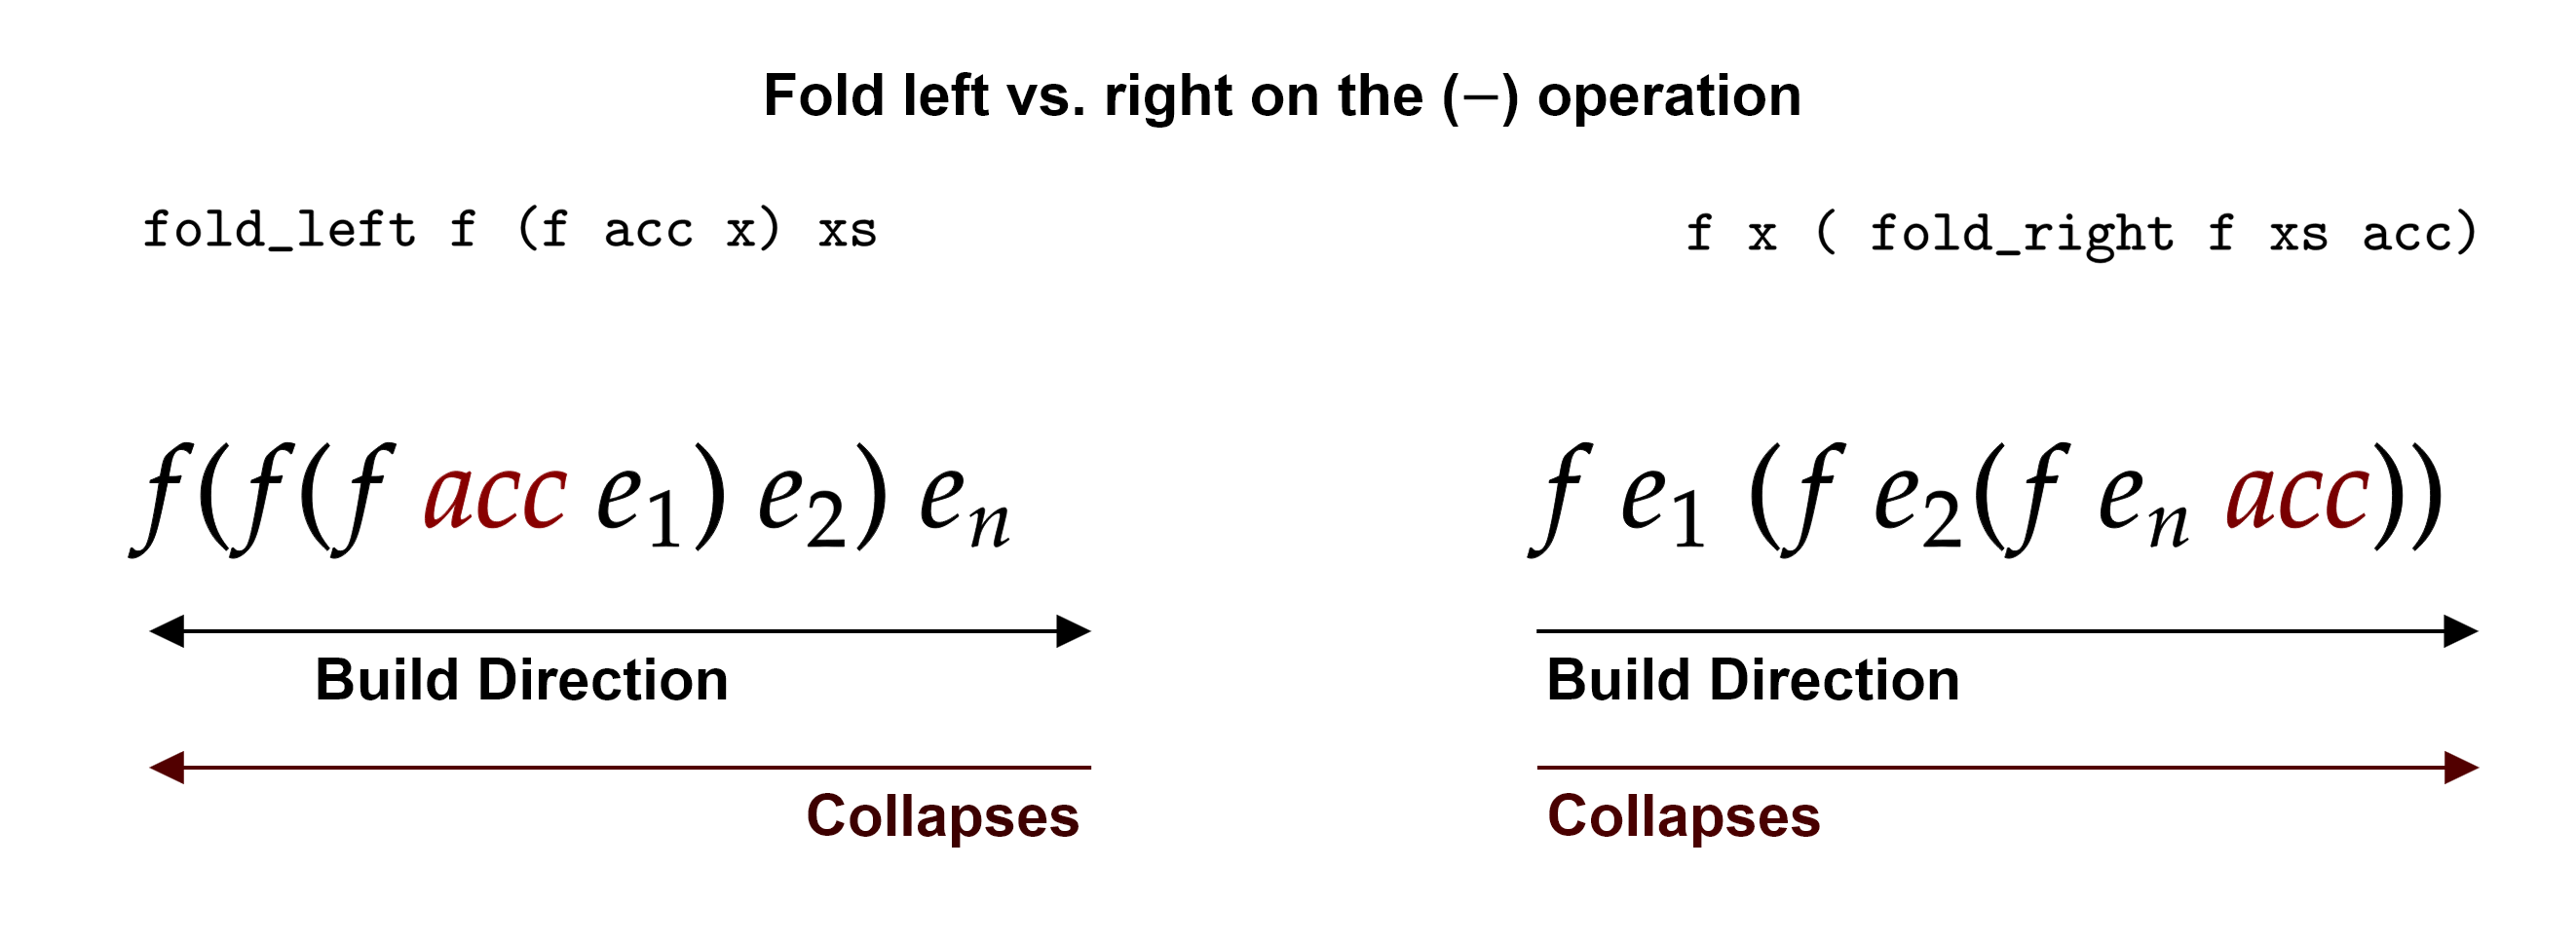
\includegraphics[width=0.8\textwidth]{Sections/order/fold.png}
    \caption{Fold Left vs. Fold Right}
\end{figure}

\noindent
In both, we still build from the base case/last element to the front of the list. So above, we are always building from right to left.
The difference: 

\begin{itemize}
    \item \textbf{Fold Left}: We tunnel in from right to left, applying the accumulator to the first element.
    \item \textbf{Fold Right}: We box up values from left to right, applying the accumulator to the last element.
\end{itemize}

\noindent
Though again for emphasis, the original naming intention was: 
\begin{itemize}
    \item \textbf{Fold Left}: Apply the accumulator from the \textbf{left} of the list to the right.
    \item \textbf{Fold Right}: Apply the accumulator from the \textbf{right} of the list to the left.
\end{itemize}



